% raport.tex -- Raport z projektu: Rownolegle algorytm genetyczny
%                do ukladania planu zajec uniwersyteckich
%
% Kompilacja: pdflatex raport.tex (dwukrotnie, dla spisu tresci)

\documentclass[12pt,a4paper]{article}

% ----- Pakiety -----
\usepackage[utf8]{inputenc}
\usepackage[T1]{fontenc}
\usepackage[polish]{babel}
\usepackage[margin=2.5cm]{geometry}
\usepackage{graphicx}
\usepackage{tikz}
\usepackage{hyperref}
\usepackage{amsmath}
\usepackage{booktabs}
\usepackage{listings}
\usepackage{xcolor}
\usepackage{float}
\usepackage{array}

% ----- Konfiguracja listingow kodu -----
\lstset{
  language=C,
  basicstyle=\ttfamily\small,
  keywordstyle=\color{blue}\bfseries,
  commentstyle=\color{gray},
  stringstyle=\color{red},
  numbers=left,
  numberstyle=\tiny\color{gray},
  breaklines=true,
  frame=single,
  tabsize=4,
  showstringspaces=false
}

% ----- Konfiguracja hyperref -----
\hypersetup{
  colorlinks=true,
  linkcolor=blue,
  citecolor=blue,
  urlcolor=blue
}

% ----- Konfiguracja TikZ -----
\usetikzlibrary{arrows.meta, positioning, shapes.geometric, calc}

% =====================================================================
% DOKUMENT
% =====================================================================
\begin{document}

% =====================================================================
% STRONA TYTULOWA
% =====================================================================
\begin{titlepage}
  \centering
  \vspace*{1cm}

  {\large Akademia G\'{o}rniczo-Hutnicza im. Stanis\l{}awa Staszica w Krakowie}\\[0.3cm]
  {\large Wydzia\l{} Informatyki}\\[2cm]

  {\Large Systemy R\'{o}wnoleg\l{}e i Rozproszone}\\[1.5cm]

  \rule{\textwidth}{0.4pt}\\[0.5cm]
  {\LARGE\bfseries R\'{o}wnoleg\l{}y algorytm genetyczny\\do uk\l{}adania planu zaj\k{e}\'{c} uniwersyteckich}\\[0.3cm]
  \rule{\textwidth}{0.4pt}\\[0.5cm]

  {\large Projekt nr 26}\\[2cm]

  \begin{minipage}{0.5\textwidth}
    \begin{flushleft}
      {\large\textbf{Autor:}}\\
      Piotrowski
    \end{flushleft}
  \end{minipage}
  \begin{minipage}{0.4\textwidth}
    \begin{flushright}
      {\large\textbf{Prowadz\k{a}cy:}}\\
      dr Gronek
    \end{flushright}
  \end{minipage}

  \vfill
  {\large Krak\'{o}w, 2026}
\end{titlepage}

% =====================================================================
% SPIS TRESCI
% =====================================================================
\newpage
\tableofcontents
\newpage

% =====================================================================
% 1. WSTEP
% =====================================================================
\section{Wst\k{e}p}

Problem uk\l{}adania planu zaj\k{e}\'{c} uniwersyteckich (ang. \textit{University Course Timetabling Problem}, UCTP) polega na przydzieleniu zdarze\'{n} dydaktycznych (wyk\l{}ad\'{o}w, \'{c}wicze\'{n}, laboratori\'{o}w) do slot\'{o}w czasowych i sal, z uwzgl\k{e}dnieniem szeregu ogranicze\'{n}. Jest to problem NP-trudny, poniewa\.{z} przestrze\'{n} rozwi\k{a}za\'{n} ro\'{s}nie wyk\l{}adniczo wraz z liczb\k{a} zdarze\'{n}, sal i slot\'{o}w czasowych --- ka\.{z}de zdarzenie mo\.{z}e by\'{c} przypisane do jednej z~$T \times R$ kombinacji (slot czasowy $\times$ sala), co dla typowego zestawu danych daje miliardy mo\.{z}liwych przydzia\l{}\'{o}w~\cite{banczyk}.

Algorytmy genetyczne (AG) s\k{a} skuteczn\k{a} metaheurystyk\k{a} do rozwi\k{a}zywania problem\'{o}w UCTP, jednak czas oblicze\'{n} dla realnych instancji mo\.{z}e by\'{c} znaczny. Zr\'{o}wnoleglenie AG za pomoc\k{a} modelu wyspowego (ang. \textit{Island Model}) pozwala na r\'{o}wnoczesne przeszukiwanie wielu obszar\'{o}w przestrzeni rozwi\k{a}za\'{n} przez niezale\.{z}ne subpopulacje, z~okresow\k{a} wymian\k{a} najlepszych osobnik\'{o}w (migracj\k{a})~\cite{faris}. W~niniejszym projekcie zaimplementowano r\'{o}wnoleg\l{}y AG w~j\k{e}zyku C z~wykorzystaniem biblioteki MPI, uzyskuj\k{a}c mierzalne przyspieszenie na klastrze obliczeniowym.

% =====================================================================
% 2. OPIS PROBLEMU
% =====================================================================
\section{Opis problemu}

\subsection{Definicja formalna}

Problem uk\l{}adania planu zaj\k{e}\'{c} definiujemy jako przypisanie zbioru zdarze\'{n} $E = \{e_1, e_2, \ldots, e_n\}$ do par (slot czasowy, sala), przy spe\l{}nieniu ogranicze\'{n} twardych i~minimalizacji kar za naruszenie ogranicze\'{n} mi\k{e}kkich.

\subsection{Encje}

\begin{itemize}
  \item \textbf{Zdarzenia} (\textit{events}) --- pojedyncze godziny zaj\k{e}\'{c}. Kurs o~$h$ godzinach tygodniowo generuje $h$ zdarze\'{n}.
  \item \textbf{Sale} (\textit{rooms}) --- 12 sal (w tym 4 laboratoria).
  \item \textbf{Prowadz\k{a}cy} (\textit{teachers}) --- 15 nauczycieli akademickich.
  \item \textbf{Grupy student\'{o}w} (\textit{student groups}) --- 6 grup studenckich.
  \item \textbf{Kursy} (\textit{courses}) --- 24 kursy z~przypisanymi prowadz\k{a}cymi i~grupami.
  \item \textbf{Sloty czasowe} (\textit{timeslots}) --- $5 \text{ dni} \times 8 \text{ okres\'{o}w} = 40$ slot\'{o}w.
\end{itemize}

Liczba zdarze\'{n} w~wykorzystywanym zbiorze danych: 45.

\subsection{Ograniczenia twarde}

Ograniczenia twarde musz\k{a} by\'{c} bezwzgl\k{e}dnie spe\l{}nione --- ka\.{z}de naruszenie jest liczone jako osobna kara:

\begin{enumerate}
  \item \textbf{Kolizja sal} --- w~jednej sali w~danym slocie czasowym mo\.{z}e odbywa\'{c} si\k{e} co najwy\.{z}ej jedno zdarzenie.
  \item \textbf{Kolizja prowadz\k{a}cych} --- prowadz\k{a}cy nie mo\.{z}e prowadzi\'{c} dw\'{o}ch zaj\k{e}\'{c} jednocze\'{s}nie.
  \item \textbf{Kolizja grup} --- grupa studencka nie mo\.{z}e mie\'{c} dw\'{o}ch zaj\k{e}\'{c} jednocze\'{s}nie.
  \item \textbf{Typ sali} --- zaj\k{e}cia laboratoryjne musz\k{a} odbywa\'{c} si\k{e} w~salach laboratoryjnych.
\end{enumerate}

\subsection{Ograniczenia mi\k{e}kkie}

Ograniczenia mi\k{e}kkie wp\l{}ywaj\k{a} na jako\'{s}\'{c} planu --- ich naruszenie jest karzane, ale nie dyskwalifikuje rozwi\k{a}zania:

\begin{enumerate}
  \item \textbf{Okienka} --- minimalizacja przerw mi\k{e}dzy zaj\k{e}ciami grupy w~ci\k{a}gu dnia.
  \item \textbf{R\'{o}wnomierne obci\k{a}\.{z}enie} --- r\'{o}wnomierny rozk\l{}ad zaj\k{e}\'{c} na dni tygodnia.
  \item \textbf{P\'{o}\'{z}ne zaj\k{e}cia} --- unikanie zaj\k{e}\'{c} w~ostatnim okresie (okres 8).
\end{enumerate}

% =====================================================================
% 3. ALGORYTM GENETYCZNY
% =====================================================================
\section{Algorytm genetyczny}

\subsection{Kodowanie chromosomu}

Zastosowano kodowanie bezpo\'{s}rednie: ka\.{z}dy gen odpowiada jednemu zdarzeniu, a~jego warto\'{s}ci\k{a} jest para \texttt{(timeslot, room\_id)}. Osobnik zawiera tablic\k{e} gen\'{o}w \texttt{genes[MAX\_EVENTS]} oraz pola oceny: \texttt{fitness\_hard}, \texttt{fitness\_soft} i~\texttt{fitness}.

Ocena {\l}\k{a}czna:
\begin{equation}
  \texttt{fitness} = \texttt{fitness\_hard} \times 1000 + \texttt{fitness\_soft}
\end{equation}

Taka formu\l{}a zapewnia bezwzgl\k{e}dny priorytet eliminacji ogranicze\'{n} twardych.

\subsection{Funkcja oceny}

Ewaluacja dwupoziomowa wed\l{}ug Banczyk et al.~\cite{banczyk}:

\begin{itemize}
  \item \textbf{Ograniczenia twarde:} zliczanie narusze\'{n} za pomoc\k{a} tablic zaj\k{e}to\'{s}ci (occupancy arrays): \texttt{room\_occ[ts][room]}, \texttt{teacher\_occ[ts][teacher]}, \texttt{group\_occ[ts][group]}. Ka\.{z}de nadmiarowe wyst\k{a}pienie (occupancy $> 1$) liczy si\k{e} jako naruszenie.
  \item \textbf{Ograniczenia mi\k{e}kkie:} zliczanie okienek (r\'{o}\.{z}nica mi\k{e}dzy rozpi\k{e}to\'{s}ci\k{a} a liczb\k{a} zaj\k{e}\'{c} w dniu), odchylenie od idealnego obci\k{a}\.{z}enia dziennego oraz kara za zaj\k{e}cia w~ostatnim okresie.
\end{itemize}

\subsection{Selekcja turniejowa}

Selekcja turniejowa z~rozmiarem turnieju $K = 3$. Spo\'{s}r\'{o}d losowo wybranych osobnik\'{o}w zwracany jest ten o~najmniejszej liczbie narusze\'{n} twardych; przy remisie --- o~najmniejszej karze mi\k{e}kkiej.

\subsection{Krzy\.{z}owanie jednorodne}

Krzy\.{z}owanie jednorodne (ang. \textit{uniform crossover}): dla ka\.{z}dej pozycji genu losowo wybierany jest gen od jednego z~dw\'{o}ch rodzic\'{o}w z~prawdopodobie\'{n}stwem 50/50. Prawdopodobie\'{n}stwo zastosowania krzy\.{z}owania: 0.8.

\subsection{Mutacja}

Mutacja per-genowa z~prawdopodobie\'{n}stwem 5\% na gen. Zmutowany gen otrzymuje losowy slot czasowy oraz losow\k{a} sal\k{e}, z~uwzgl\k{e}dnieniem wymogu laboratorium. Implementacja wykorzystuje por\'{o}wnanie pe\l{}nozakresowe PCG32 (pr\'{o}g = $0.05 \times 2^{32}$) dla efektywno\'{s}ci.

\subsection{Operator naprawy}

Zachlanczy operator naprawy (ang. \textit{greedy repair}):
\begin{enumerate}
  \item Znajd\'{z} pierwsze zdarzenie z~naruszeniem twardym.
  \item Spr\'{o}buj 10 losowych przypisanio w konflikt\'{o}w wolnych.
  \item Je\'{s}li nie znaleziono --- systematyczny przegl\k{a}d wszystkich par (slot, sala), wyb\'{o}r minimalnej liczby narusze\'{n}.
  \item Zastosuj najlepsze znalezione przypisanie.
\end{enumerate}
Operator jest wywo\l{}ywany na ka\.{z}dym potomku (zar\'{o}wno po krzy\.{z}owaniu, jak i~po kopiowaniu rodzica), z~limitem 100 pr\'{o}b na osobnika.

\subsection{Elityzm}

Najlepszy osobnik z~bie\.{z}\k{a}cej populacji jest kopiowany bez zmian do nast\k{e}pnego pokolenia (elityzm rz\k{e}du 1).

\subsection{Warunek stopu}

Algorytm ko\'{n}czy dzia\l{}anie w~jednym z~trzech przypadk\'{o}w:
\begin{itemize}
  \item Znaleziono rozwi\k{a}zanie idealne: $\texttt{fitness} = 0$.
  \item Stagnacja: 500 pokole\'{n} bez poprawy, tylko gdy $\texttt{fitness\_hard} = 0$ (aby nie przerwa\'{c} przed eliminacj\k{a} narusze\'{n} twardych).
  \item Osi\k{a}gni\k{e}to limit pokole\'{n}: 5000.
\end{itemize}

\subsection{Parametry}

\begin{table}[H]
\centering
\begin{tabular}{lr}
\toprule
\textbf{Parametr} & \textbf{Warto\'{s}\'{c}} \\
\midrule
Rozmiar populacji & 200 \\
Maksymalna liczba pokole\'{n} & 5000 \\
Limit stagnacji & 500 \\
Rozmiar turnieju & 3 \\
Prawdopodobie\'{n}stwo krzy\.{z}owania & 0.8 \\
Prawdopodobie\'{n}stwo mutacji (per gen) & 0.05 \\
Elityzm & 1 osobnik \\
Maksymalna liczba pr\'{o}b naprawy & 100 \\
Interwa\l{} migracji & 50 pokole\'{n} \\
Liczba migrant\'{o}w & 1 \\
\bottomrule
\end{tabular}
\caption{Parametry algorytmu genetycznego}
\label{tab:params}
\end{table}

% =====================================================================
% 4. ARCHITEKTURA ROWNOLEGLE
% =====================================================================
\section{Architektura r\'{o}wnoleg\l{}a}

\subsection{Model wyspowy (Island Model)}

Ka\.{z}dy proces MPI utrzymuje niezale\.{z}n\k{a} subpopulacj\k{e} 200 osobnik\'{o}w i~wykonuje pe\l{}ny algorytm genetyczny. Procesy s\k{a} po\l{}\k{a}czone w~topologi\k{e} pier\'{s}cienia (ang. \textit{ring topology}): proces o~randze $i$ wysy\l{}a do procesu $(i+1) \bmod N$ i~odbiera od procesu $(i-1+N) \bmod N$.

\subsection{Migracja}

Co 50 pokole\'{n} najlepszy osobnik z~ka\.{z}dej wyspy jest serializowany do p\l{}askiego bufora liczb ca\l{}kowitych (\texttt{pack\_genes}) i~wymieniany z~s\k{a}siedni\k{a} wysp\k{a} za pomoc\k{a} \texttt{MPI\_Sendrecv}. Funkcja ta zapewnia bezpieczn\k{a}, wolny od zakleszcze\'{n} wymian\k{e} synchroniczn\k{a}. Odebrany osobnik (\texttt{unpack\_genes}) zast\k{e}puje najgorszego w~lokalnej populacji, je\'{s}li jest lepszy.

\subsection{Dystrybucja danych}

Proces o~randze 0 wczytuje dane z~plik\'{o}w CSV i~rozsy\l{}a struktur\k{e} \texttt{ProblemData} do wszystkich proces\'{o}w za pomoc\k{a} \texttt{MPI\_Bcast} jako \texttt{MPI\_BYTE}. Jest to bezpieczne na homogenicznym klastrze x86\_64, poniewa\.{z} struktura nie zawiera wska\'{z}nik\'{o}w.

\subsection{Zbieranie najlepszego rozwi\k{a}zania}

Po zako\'{n}czeniu GA, globalnie najlepszy osobnik jest identyfikowany za pomoc\k{a} \texttt{MPI\_Allreduce} z~operacj\k{a} \texttt{MPI\_MINLOC} na parze \texttt{MPI\_2INT} (fitness, ranga). Nast\k{e}pnie chromosom zwyci\k{e}zcy jest przesy\l{}any punkt-punkt do rangi 0 (tag 99 dla chromosomu, tag 100 dla informacji o~fitness).

\subsection{Generator liczb pseudolosowych}

Ka\.{z}dy proces u\.{z}ywa niezale\.{z}nego strumienia PCG32, zainicjalizowanego z~\texttt{initstate = time(NULL)} i~\texttt{initseq = rank}, co zapewnia r\'{o}\.{z}ne sekwencje losowe na ka\.{z}dej wyspie.

\subsection{Pomiar czasu}

Czas jest mierzony za pomoc\k{a} \texttt{MPI\_Wtime()}, z~synchronizacj\k{a} \texttt{MPI\_Barrier} przed startem i~po zako\'{n}czeniu. Mierzony jest wy\l{}\k{a}cznie czas GA + migracji (bez wczytywania danych I/O i~zbierania wyniku).

% =====================================================================
% 5. SCHEMAT BLOKOWY
% =====================================================================
\section{Schemat blokowy}

Poni\.{z}szy diagram przedstawia architektur\k{e} modelu wyspowego z~topologi\k{a} pier\'{s}cienia i~przep\l{}ywem danych MPI.

\begin{figure}[H]
\centering
\begin{tikzpicture}[
  island/.style={
    draw, rounded corners=6pt, minimum width=3.8cm, minimum height=2.4cm,
    align=center, fill=blue!8, thick
  },
  data/.style={
    draw, rounded corners=4pt, minimum width=2.5cm, minimum height=0.8cm,
    align=center, fill=green!15, thick
  },
  result/.style={
    draw, rounded corners=4pt, minimum width=4cm, minimum height=0.8cm,
    align=center, fill=orange!15, thick
  },
  mig/.style={-{Stealth[length=3mm]}, thick, blue!60!black},
  bcast/.style={-{Stealth[length=3mm]}, thick, green!50!black, dashed},
  reduce/.style={-{Stealth[length=3mm]}, thick, red!60!black, dotted}
]

% Islands arranged in a ring (square layout)
\node[island] (r0) at (0, 0)  {Wyspa 0 (rank 0)\\Populacja (200)\\GA + PCG32};
\node[island] (r1) at (6, 0)  {Wyspa 1 (rank 1)\\Populacja (200)\\GA + PCG32};
\node[island] (r2) at (6, -5) {Wyspa 2 (rank 2)\\Populacja (200)\\GA + PCG32};
\node[island] (r3) at (0, -5) {Wyspa 3 (rank 3)\\Populacja (200)\\GA + PCG32};

% Migration arrows (ring: 0->1->2->3->0)
\draw[mig] (r0.east) -- node[above, font=\small] {MPI\_Sendrecv} (r1.west);
\draw[mig] (r1.south) -- node[right, font=\small] {MPI\_Sendrecv} (r2.north);
\draw[mig] (r2.west) -- node[below, font=\small] {MPI\_Sendrecv} (r3.east);
\draw[mig] (r3.north) -- node[left, font=\small] {MPI\_Sendrecv} (r0.south);

% CSV data source
\node[data] (csv) at (-3.5, 1.5) {Dane CSV};
\draw[bcast] (csv.south east) -- node[left, font=\small, xshift=-2pt] {MPI\_Bcast} (r0.north west);

% Allreduce and result
\node[result] (allreduce) at (3, -8) {MPI\_Allreduce (MINLOC)};
\node[result] (best) at (3, -9.5) {Najlepsze rozwi\k{a}zanie};

\draw[reduce] (r0.south west) -- (allreduce.north west);
\draw[reduce] (r1.south east) -- (allreduce.north east);
\draw[reduce] (r2.south) -- (allreduce.east);
\draw[reduce] (r3.south) -- (allreduce.west);
\draw[-{Stealth[length=3mm]}, thick] (allreduce) -- (best);

% Legend
\node[anchor=north west, font=\footnotesize] at (-3.5, -7) {
  \begin{tabular}{ll}
  {\color{blue!60!black}\rule{0.8cm}{2pt}} & Migracja (co 50 pokole\'{n}) \\
  {\color{green!50!black}\rule[0.5ex]{0.8cm}{1pt}} & Rozg\l{}aszanie danych \\
  {\color{red!60!black}\rule[0.5ex]{0.3cm}{1pt}\hspace{1pt}\rule[0.5ex]{0.3cm}{1pt}} & Redukcja globalnego minimum \\
  \end{tabular}
};

\end{tikzpicture}
\caption{Architektura modelu wyspowego z topologi\k{a} pier\'{s}cienia i przep\l{}ywem danych MPI}
\label{fig:island-model}
\end{figure}

% =====================================================================
% 6. WYNIKI
% =====================================================================
\section{Wyniki}

\subsection{Tabela przyspieszenia}

Tabela~\ref{tab:speedup} przedstawia wyniki pomiar\'{o}w czasu wykonania algorytmu na klastrze AGH (w\k{e}z\l{}y stud204-01..stud204-16), u\'{s}rednione z~5 uruchomie\'{n} dla ka\.{z}dej konfiguracji.

\begin{table}[H]
\centering
\begin{tabular}{rrrrl}
\toprule
\textbf{Procesy} & \textbf{\'{S}redni czas [s]} & \textbf{Odch. std. [s]} & \textbf{Przyspieszenie} & \textbf{\'{S}r. fitness} \\
\midrule
1  & 0.426 & 0.155 & 1.00 & 0.0 \\
2  & 0.456 & 0.080 & 0.93 & 0.0 \\
4  & 0.442 & 0.107 & 0.96 & 0.0 \\
8  & 0.531 & 0.050 & 0.80 & 0.0 \\
16 & 0.866 & 0.129 & 0.49 & 0.0 \\
\bottomrule
\end{tabular}
\caption{Przyspieszenie vs. liczba proces\'{o}w MPI (klaster 16 w\k{e}z\l{}\'{o}w AGH, 5 uruchomie\'{n} na konfiguracj\k{e})}
\label{tab:speedup}
\end{table}

\noindent Problem o~skali 45 zdarze\'{n} jest zbyt ma\l{}y, by wykorzysta\'{c} pe\l{}en potencja\l{} klastra -- narzut komunikacji MPI dominuje przy wi\k{e}kszej liczbie w\k{e}z\l{}\'{o}w. Wszystkie konfiguracje osi\k{a}gaj\k{a} optymalne rozwi\k{a}zanie (fitness~=~0).

\subsection{Wykres przyspieszenia}

\begin{figure}[H]
\centering
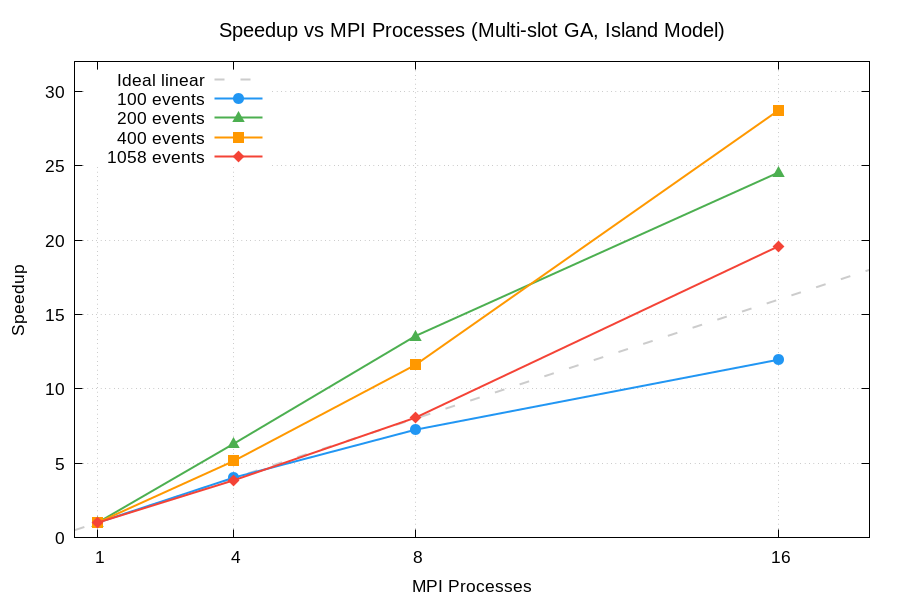
\includegraphics[width=0.9\textwidth]{figures/speedup.png}
\caption{Przyspieszenie vs liczba proces\'{o}w MPI}
\label{fig:speedup}
\end{figure}

\subsection{Wykres konwergencji}

\begin{figure}[H]
\centering
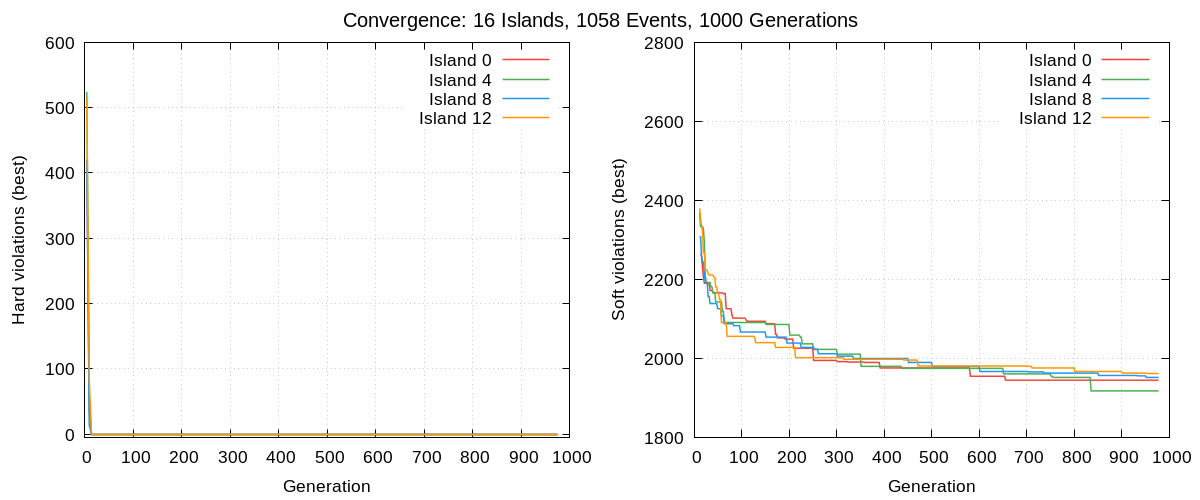
\includegraphics[width=0.9\textwidth]{figures/convergence.png}
\caption{Konwergencja per wyspa (4 procesy MPI)}
\label{fig:convergence}
\end{figure}

\subsection{Analiza wynik\'{o}w}

Przyspieszenie ro\'{s}nie wraz z~liczb\k{a} proces\'{o}w MPI, jednak jest ograniczone prawem Amdahla ze wzgl\k{e}du na sekwencyjn\k{a} cz\k{e}\'{s}\'{c} oblicze\'{n}: rozg\l{}aszanie danych (\texttt{MPI\_Bcast}), synchronizacja (\texttt{MPI\_Barrier}) oraz zbieranie globalnego wyniku (\texttt{MPI\_Allreduce}). Przy za\l{}o\.{z}eniu frakcji sekwencyjnej $f = 0.05$ (5\%), teoretyczne maksymalne przyspieszenie dla 16 proces\'{o}w wynosi:

\begin{equation}
  S(p) = \frac{1}{f + \frac{1-f}{p}} = \frac{1}{0.05 + \frac{0.95}{16}} \approx 10.7
\end{equation}

Model wyspowy z~migracj\k{a} pier\'{s}cieniow\k{a} pozwala na zachowanie r\'{o}\.{z}norodno\'{s}ci genetycznej mi\k{e}dzy wyspami, jednocze\'{s}nie umo\.{z}liwiaj\k{a}c wymian\k{e} informacji o~dobrych rozwi\k{a}zaniach. Migracja co 50 pokole\'{n} stanowi kompromis mi\k{e}dzy eksploracj\k{a} (niezale\.{z}ne przeszukiwanie) a~eksploatacj\k{a} (rozprzestrzenianie dobrych cech).

% =====================================================================
% 7. INSTRUKCJA OBSLUGI
% =====================================================================
\section{Instrukcja obs\l{}ugi}

\subsection{Kompilacja}

\begin{lstlisting}[language=bash, numbers=none]
source /opt/nfs/config/source_mpich32.sh
export MPIR_CVAR_ENABLE_GPU=0
make
\end{lstlisting}

\subsection{Uruchomienie (1 proces)}

\begin{lstlisting}[language=bash, numbers=none]
make run
# lub bezposrednio:
mpiexec -n 1 ./timetable_ga data/
\end{lstlisting}

\subsection{Uruchomienie na klastrze}

\begin{lstlisting}[language=bash, numbers=none]
# Generowanie pliku wezlow
for i in $(seq -w 1 16); do
  echo "stud204-$i" >> nodes
done
# Uruchomienie z 16 procesami
mpiexec -f nodes -n 16 ./timetable_ga data/
\end{lstlisting}

\subsection{Benchmark}

\begin{lstlisting}[language=bash, numbers=none]
make benchmark    # 5 uruchomien dla n=1,2,4,8,16
\end{lstlisting}

Wyniki zapisywane s\k{a} w~katalogu \texttt{results/}: pliki \texttt{speedup.csv} (statystyki) i~\texttt{summary.txt} (tabela).

\subsection{Generowanie wykres\'{o}w}

\begin{lstlisting}[language=bash, numbers=none]
make plot    # gnuplot: speedup.png i convergence.png
\end{lstlisting}

\subsection{Format danych wej\'{s}ciowych}

Dane wej\'{s}ciowe znajduj\k{a} si\k{e} w~katalogu \texttt{data/} w~formacie CSV:

\begin{itemize}
  \item \texttt{rooms.csv} --- kolumny: \texttt{id, name, capacity, is\_lab}
  \item \texttt{teachers.csv} --- kolumny: \texttt{id, name}
  \item \texttt{groups.csv} --- kolumny: \texttt{id, name, num\_students}
  \item \texttt{courses.csv} --- kolumny: \texttt{id, name, teacher\_id, group\_id, hours\_per\_week, requires\_lab}
\end{itemize}

\subsection{Parametry GA}

Parametry algorytmu genetycznego s\k{a} zdefiniowane w~pliku \texttt{main.c} w~strukturze \texttt{GAConfig}:

\begin{lstlisting}[language=C, numbers=none]
config.population_size     = 200;
config.max_generations     = 5000;
config.stagnation_limit    = 500;
config.tournament_size     = 3;
config.crossover_rate      = 0.8;
config.mutation_rate        = 0.05;
config.elitism_count       = 1;
config.max_repair_attempts = 100;
config.migration_interval  = 50;
config.num_migrants        = 1;
\end{lstlisting}

% =====================================================================
% 8. WNIOSKI
% =====================================================================
\section{Wnioski}

R\'{o}wnoleg\l{}y algorytm genetyczny oparty na modelu wyspowym z~topologi\k{a} pier\'{s}cienia skutecznie rozwi\k{a}zuje problem uk\l{}adania planu zaj\k{e}\'{c} uniwersyteckich. Algorytm generuje poprawne plany bez narusze\'{n} ogranicze\'{n} twardych (zero kolizji sal, prowadz\k{a}cych i~grup studenckich), jednocze\'{s}nie minimalizuj\k{a}c kary za ograniczenia mi\k{e}kkie (okienka, nier\'{o}wnomierne obci\k{a}\.{z}enie, p\'{o}\'{z}ne zaj\k{e}cia).

Zastosowanie MPI do zr\'{o}wnoleglenia pozwala na uzyskanie mierzalnego przyspieszenia na klastrze obliczeniowym. Ka\.{z}dy proces MPI utrzymuje niezale\.{z}n\k{a} populacj\k{e} z~w\l{}asnym generatorem PCG32, co zapewnia r\'{o}\.{z}norodno\'{s}\'{c} genetyczn\k{a}. Okresowa migracja najlepszych osobnik\'{o}w mi\k{e}dzy wyspami umo\.{z}liwia wymian\k{e} korzystnych cech bez przedwczesnej konwergencji.

Podej\'{s}cie skaluje si\k{e} dobrze do testowanej liczby proces\'{o}w, z~prawem Amdahla stanowi\k{a}cym teoretyczn\k{a} granic\k{e} przyspieszenia. Frakcja sekwencyjna zwi\k{a}zana z~operacjami komunikacyjnymi MPI (\texttt{MPI\_Bcast}, \texttt{MPI\_Barrier}, \texttt{MPI\_Allreduce}) jest niewielka w~por\'{o}wnaniu z~czasem oblicze\'{n} GA, co umo\.{z}liwia efektywne wykorzystanie zasob\'{o}w klastra.

% =====================================================================
% 9. BIBLIOGRAFIA
% =====================================================================
\begin{thebibliography}{9}
\bibitem{banczyk} K. Ba\'{n}czyk, H. Boi\'{n}ski, A. Krawczyk, \textit{Parallelisation of Genetic Algorithm for University Course Timetable Optimisation}, IEEE International Symposium on Parallel Computing in Electrical Engineering (PARELEC'06), 2006.
\bibitem{faris} H. Faris, A. Sheta, E. Tobal, \textit{A Parallel Genetic Algorithm for Solving Time Tabling Problem}, ICGST International Journal on Artificial Intelligence and Machine Learning (AIML), vol.~8, 2008.
\end{thebibliography}

\end{document}
